% Options for packages loaded elsewhere
\PassOptionsToPackage{unicode}{hyperref}
\PassOptionsToPackage{hyphens}{url}
%
\documentclass[
]{article}
\usepackage{lmodern}
\usepackage{amssymb,amsmath}
\usepackage{ifxetex,ifluatex}
\ifnum 0\ifxetex 1\fi\ifluatex 1\fi=0 % if pdftex
  \usepackage[T1]{fontenc}
  \usepackage[utf8]{inputenc}
  \usepackage{textcomp} % provide euro and other symbols
\else % if luatex or xetex
  \usepackage{unicode-math}
  \defaultfontfeatures{Scale=MatchLowercase}
  \defaultfontfeatures[\rmfamily]{Ligatures=TeX,Scale=1}
\fi
% Use upquote if available, for straight quotes in verbatim environments
\IfFileExists{upquote.sty}{\usepackage{upquote}}{}
\IfFileExists{microtype.sty}{% use microtype if available
  \usepackage[]{microtype}
  \UseMicrotypeSet[protrusion]{basicmath} % disable protrusion for tt fonts
}{}
\makeatletter
\@ifundefined{KOMAClassName}{% if non-KOMA class
  \IfFileExists{parskip.sty}{%
    \usepackage{parskip}
  }{% else
    \setlength{\parindent}{0pt}
    \setlength{\parskip}{6pt plus 2pt minus 1pt}}
}{% if KOMA class
  \KOMAoptions{parskip=half}}
\makeatother
\usepackage{xcolor}
\IfFileExists{xurl.sty}{\usepackage{xurl}}{} % add URL line breaks if available
\IfFileExists{bookmark.sty}{\usepackage{bookmark}}{\usepackage{hyperref}}
\hypersetup{
  pdftitle={Covid-19 Spread - Cross sectional Analysis of US Counties},
  pdfauthor={Muhammad Zargham, Clark Granger, Zachary Carlson},
  hidelinks,
  pdfcreator={LaTeX via pandoc}}
\urlstyle{same} % disable monospaced font for URLs
\usepackage[margin=1in]{geometry}
\usepackage{graphicx,grffile}
\makeatletter
\def\maxwidth{\ifdim\Gin@nat@width>\linewidth\linewidth\else\Gin@nat@width\fi}
\def\maxheight{\ifdim\Gin@nat@height>\textheight\textheight\else\Gin@nat@height\fi}
\makeatother
% Scale images if necessary, so that they will not overflow the page
% margins by default, and it is still possible to overwrite the defaults
% using explicit options in \includegraphics[width, height, ...]{}
\setkeys{Gin}{width=\maxwidth,height=\maxheight,keepaspectratio}
% Set default figure placement to htbp
\makeatletter
\def\fps@figure{htbp}
\makeatother
\setlength{\emergencystretch}{3em} % prevent overfull lines
\providecommand{\tightlist}{%
  \setlength{\itemsep}{0pt}\setlength{\parskip}{0pt}}
\setcounter{secnumdepth}{-\maxdimen} % remove section numbering
\usepackage{dcolumn}
\usepackage{graphicx}
\usepackage{setspace}
\usepackage{comment}
\usepackage{caption}
\usepackage{enumerate}
\usepackage{amsmath}
\usepackage{bbold}
\usepackage{url}
\usepackage{amssymb}
\usepackage{scalefnt}
\usepackage{multirow}
\usepackage{autobreak}
\usepackage{here}
\usepackage{geometry}

\usepackage{fancyhdr}
\thispagestyle{plain}
\pagestyle{fancy}
%\fancyhf{}
%\renewcommand{\headrulewidth}{0pt}
\headheight=15pt
\headsep=18pt
\lhead{Covid-19}
\rhead{Project: Data Mining}
\usepackage{booktabs}
\usepackage{longtable}
\usepackage{array}
\usepackage{multirow}
\usepackage{wrapfig}
\usepackage{float}
\usepackage{colortbl}
\usepackage{pdflscape}
\usepackage{tabu}
\usepackage{threeparttable}
\usepackage{threeparttablex}
\usepackage[normalem]{ulem}
\usepackage{makecell}
\usepackage{xcolor}

\title{Covid-19 Spread - Cross sectional Analysis of US Counties}
\author{Muhammad Zargham, Clark Granger, Zachary Carlson}
\date{}

\begin{document}
\maketitle

\begin{abstract}
We conduct a cross sectional analysis of Covid-19 cases as on April 30, 2019 across the US counties based on their socio-economic and geographical factors that may be important in explaining the different pace of virus spread. Along with identifying these important factors, we try to fit negative binomial, KNN and Random forest models to predict the number of covid-19 cases and to test whether incorporating these socio economic variables into our models can lead to better predictions of covid cases at county level. We find that some important socio-economic features are correlated with the number of cases and can give further insight for studying this pandemic.  
\end{abstract}
\newpage

{
\setcounter{tocdepth}{2}
\tableofcontents
}
\newpage

\hypertarget{introduction}{%
\section{Introduction}\label{introduction}}

Covid-19 or corona virus outbreak started from China at the end of Year
2020. By February 2020, cases start to appear in the United States and
spread rapidly across the country. The growth in the number of cases has
been exponential like in the case of any highly contagious disease. In
uncertain times like these, as scientists and researchers around the
world are actively working to come up with a cure, it is important to
know the factors that affect the spread of this virus to slow down its
spread and make plausible predictions about the future.

Since the first case of covid-19 was discovered in the US in Snohomish
county of Washington State, the virus has now spread to other places and
in some cities like New York and Chicago, the spread has been faster,
making them new hotspots for the virus. Even though cities like Seattle
\& Los Angeles reported their first cases quite earlier than others, we
see a slower pace of outbreak in these cities. A simple line graphs for
some counties that saw their first case of infection around the same
time shows the difference in the rate of virus spread.

\begin{figure}
\centering
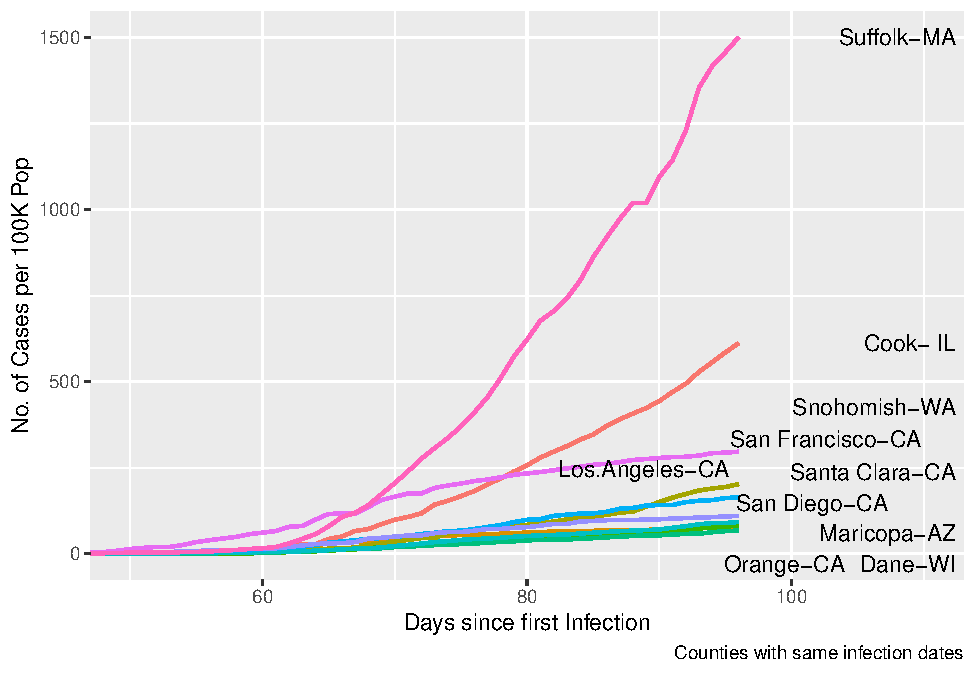
\includegraphics{Final-Project-Covid-19_files/figure-latex/unnamed-chunk-2-1.pdf}
\caption{Trend Line Graph for Counties}
\end{figure}

This poses a question: what are the different factors that are leading
to differences in the pace of covid-19 spread across the US counties?
Can a cross sectional comparison of these counties help us identify any
socio-economic or geographical features that have effect on virus spread
and can we use these features to predict the number of infections for
other counties that are behind the trend. We carry out a cross sectional
analysis of counties and their features in comparison to the number of
covid-19 cases reported by using statistical and data mining tools. The
purpose of the report is to identify any trend or characteristics of
counties that are connected to the pace of virus spread.

\hypertarget{data}{%
\section{Data}\label{data}}

\begin{itemize}
\tightlist
\item
  \textbf{Cases \& Deaths:} We collect the data of total number of
  covid-19 infection cases and deaths at county level as on April 30,
  2010. The data has been obtained from NY-Times Github repository. We
  selected 1462 counties which had non-zero number of deaths reported.
  This was done because the ACS data was only available for counties
  that have any death reported for covid-19.We divided the total number
  of cases by population to have cases per hundred thousand of
  population. This gives a good comparison of cases across counties with
  different populations. From now on we will refer to cases as cases per
  hundred thousand of population. The density graph shows that a lot of
  counties have lower number of cases and a very skewed distribution of
  cases.
\end{itemize}

\begin{figure}
\centering
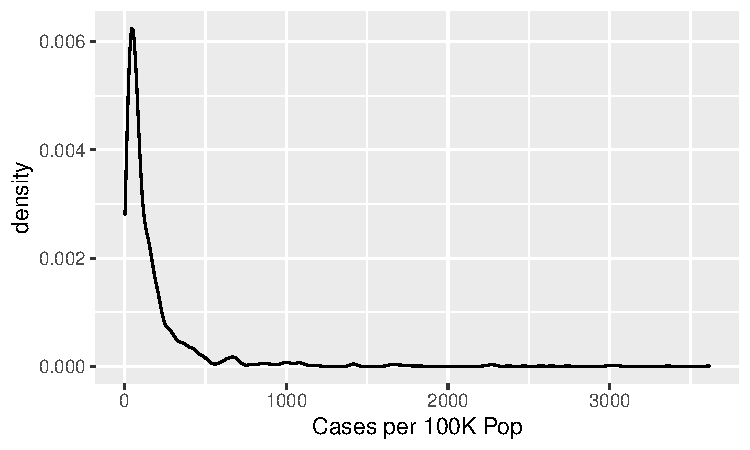
\includegraphics{Final-Project-Covid-19_files/figure-latex/unnamed-chunk-3-1.pdf}
\caption{Density Graph for Number of Cases}
\end{figure}

\begin{itemize}
\tightlist
\item
  \textbf{Days since first Case:} We calculated the total number of days
  since 1st infection for all counties as on April 30, 2020. This
  variable measures the time period for spread of virus. A scatter plot
  of days since first infection and number of cases per 100 thousand
  people shows that there is a general exponential trend but some
  counties have been able to keep their number of cases down even though
  the got the virus before other counties.
\end{itemize}

\begin{figure}
\centering
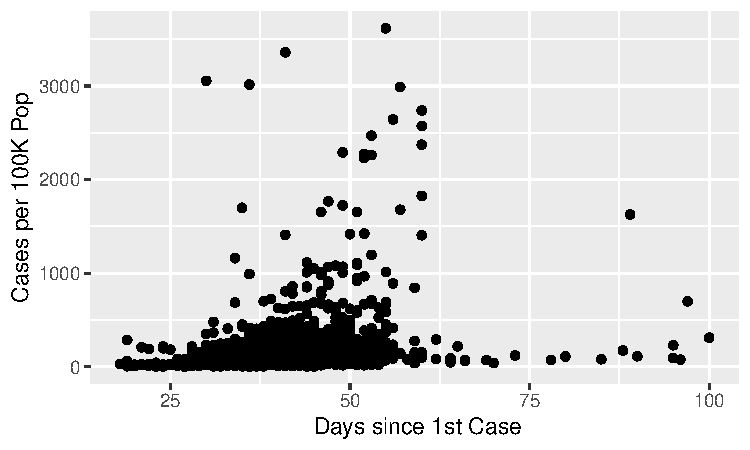
\includegraphics{Final-Project-Covid-19_files/figure-latex/unnamed-chunk-4-1.pdf}
\caption{Scatter Plot of Time and Cases}
\end{figure}

\begin{itemize}
\item
  \textbf{Days since Stay at home orders:} Similarly, we calculated
  number of days since stay at home orders were issued by State and
  County authorities as on April 30, 2020. This gives us the time period
  for interventions taken by authorities. This information was obtained
  from
  \href{https://github.com/JieYingWu/COVID-19_US_County-level_Summaries}{Jie
  Ying Wu} github respository. Along with this we also obtained Google's
  movement analytics for each county which gives a percentage decline in
  people's movement from the baseline average.
\item
  \textbf{Socio-Economic Variables:} We obtained socio economic
  variables on the population of counties from American Community Survey
  reports available on github repositories for Covid data. Main
  variables include: Unemployment rate, \% of White, \% of Households in
  Poverty, \% of population employed in different industries, median
  income and \% of population with a bachelor's degree.
\item
  \textbf{Demographic Variables:} \% of male, \% of age between 18 and
  64, \% of White, Median age, \% of total households as family etc. The
  complete list is attached in the appendix.
\item
  \textbf{Geographical variables:} We also gathered variables like
  population density, average of last 8 years highest summer temperature
  and humidity rate. We wanted to obtain the recent monthly averages for
  counties but could not find the latest data, so we used these
  variables.
\end{itemize}

There were many socio-economic variables that were very highly
correlated, so we dropped some variables and finalized 30 variables for
this analysis. The complete list of these variables is provided in the
appendix.

\textbf{Note:} Before we start with our analysis, it is important that
we acknowledge that number of cases reported depends heavily on the
number of tests conducted. Unfortunately, testing policy has not been
uniformed across US and that can lead to a measurement error in cases.
Secondly, there are reports that the given time frame for start of
covid-19 is not accurate and it is presumed that covid-19 reached many
major cities of the US way before the first case was reported.

However, due to data limitation, we must assume that the official
reporting of cases represents somewhat actual position for the start of
virus infection. For testing, we tried to get data on total tests
conducted on county level but only found the data at the state level.
So, we calculated total tests conducted per hundred thousand people for
each state and then use it for each county in the respective state. This
is not perfect because we are assuming that the rate of testing is
uniform across counties in each state but we think that public health
and testing policy is same across the all counties in each state.

\hypertarget{methods-and-results}{%
\section{Methods and Results}\label{methods-and-results}}

\hypertarget{principal-component-analysis}{%
\subsection{Principal Component
Analysis}\label{principal-component-analysis}}

We use principal component analysis to summarize the variations in
correlated socio-economic factors and see if it explains differences in
covid spread. After scaling the data, we see that 90\% of variation in
30 explanatory variables can be explained by 16 principal components,
pointing towards correlation between these variables.

The biplot of main variables that contribute to variance for first two
PCs shows that PC1 captures variation in population density, time since
first case, proportion of population between 18 and 64 and change in the
movement of people to their workplaces.

\begin{figure}
\centering
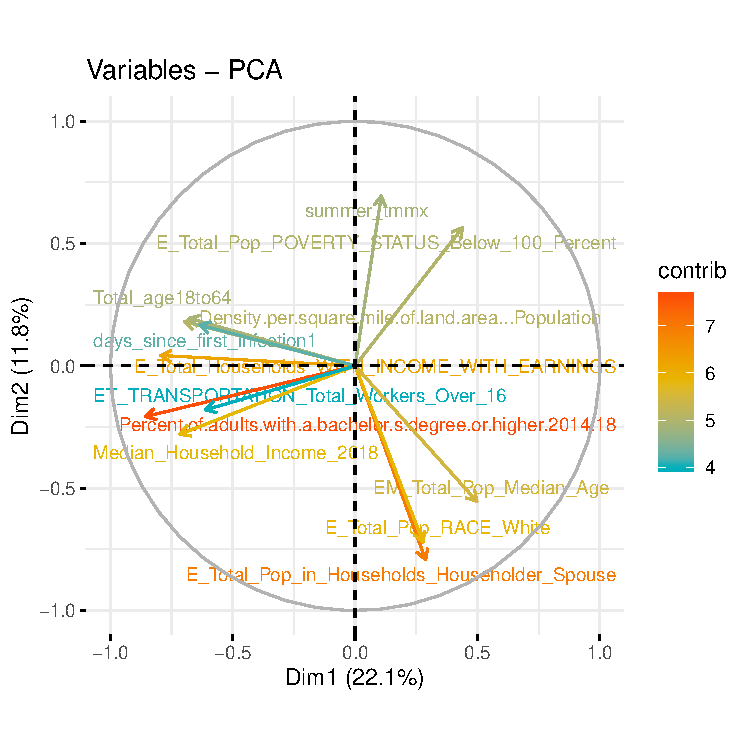
\includegraphics{Final-Project-Covid-19_files/figure-latex/unnamed-chunk-5-1.pdf}
\caption{Variables Contribution in first two PCAs}
\end{figure}

\begin{figure}
\centering
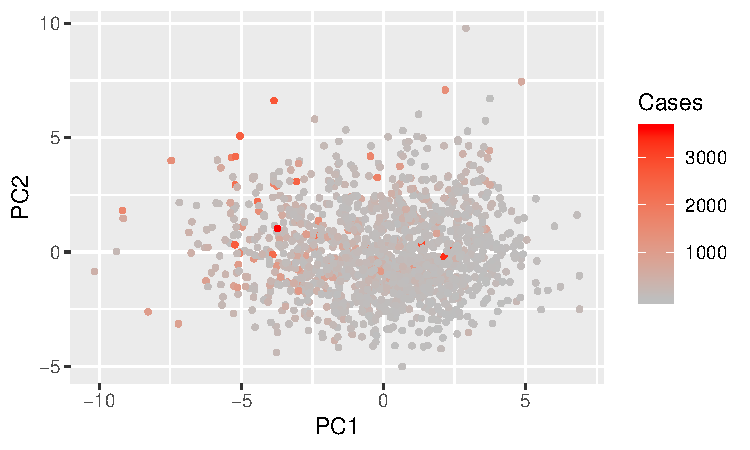
\includegraphics{Final-Project-Covid-19_files/figure-latex/unnamed-chunk-6-1.pdf}
\caption{Scatter Plot of Cases along Principal Components}
\end{figure}

Plotting the scatter plot with first two components with color scaling
the number of cases, we see that there is no tight clustering of high
case counties but generally, we see that there are more red points in
the upper left quadrant of the graph. Which means that variables
mentioned above are correlated with higher number of covid-19 cases.
Similarly, lower right quadrant has less number of high case counties
and from the biplot we saw that this is associated with higher
proportion of white population, higher median age and higher proportion
of spouse households in total households. Interestingly, we cannot say
much about the effect of temperature on virus spread but there does
seems to be a slight negative correlation between humidity level and
virus spread.

\hypertarget{negative-binomial-logistic-model}{%
\subsection{Negative Binomial Logistic
Model}\label{negative-binomial-logistic-model}}

Since our outcome is count of cases with overdispersion, we fit a
negative binomial logistic model on our data. As we have only those
counties that reported any covid cases, we use zero truncated negative
binomial logistic model. This model has been used by
\href{https://www.medrxiv.org/node/78162.external-links.html}{Wu,Nethery,Sabath
(2020)} in their study of exposure to air pollution and its effect on
covid death rate in US counties. We include all the explanatory
variables in our model to see their marginal effect on log case count.
The summary of the model is provided in the appendix.

We can clearly see that infection start date is positively correlated
with the log count of cases. Along with it, days since stay at home
orders are linked negatively to cases growth which is also theoretically
correct. Another important variable is population density per square
mile area which means that congested counties see higher number of
cases.

Counties with higher percentage of educated people and white people also
observe lower cases. People fitting the above profile are more likely to
be rich, living in large and open areas which in turn increases social
distance and lowers virus transmission. Higher proportion of people
employed in educational and health services and lower proportion of
people in arts, recreational, accommodation and public administration
industries are correlated with higher cases of virus. The signs for
these co-efficient are consistent with our PCA analysis.

We have a problem of small sample and it would have been better if the
sample size could have been bigger. We have Hauck-Donner effect in two
variables: \% of population age 18 to 64 and
E\_Total\_Households\_TYPE\_Family. The co-efficient magnitude cannot be
considered as casual effect. However, the signs of co-efficient points
towards some plausible correlation between number of cases and different
variables.

To check the predictive power of our model, we do 300 test/ train splits
of our sample and run the model. We get a RMSE of around \textbf{240}
cases per hundred thousand people. Plotting the predicted values against
the actual values, we see that the model on average underpredicts the
number of cases for counties with high number of cases and overpredicts
for counties with lower number of cases. Overall, we do not think this
model does a good job at prediction.

\begin{figure}
\centering
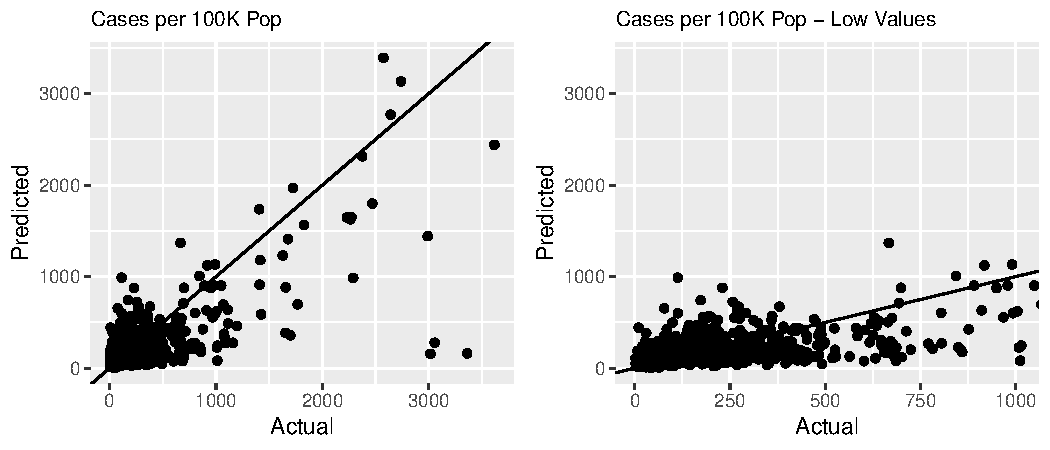
\includegraphics{Final-Project-Covid-19_files/figure-latex/unnamed-chunk-9-1.pdf}
\caption{Fitted vs Actual Cases per 100K Pop}
\end{figure}

We try the same model with actual number of cases rather than number of
cases per hundred thousand people and include log of population in the
model to control for community size. The RMSE of 300 test and train
split comes out to be around \textbf{1500} and the prediction graph is
more balanced as compared to the model with cases per hundred thousand
population. Therefore, we would prefer using total number of cases in
the model for prediction purposes.

\begin{figure}
\centering
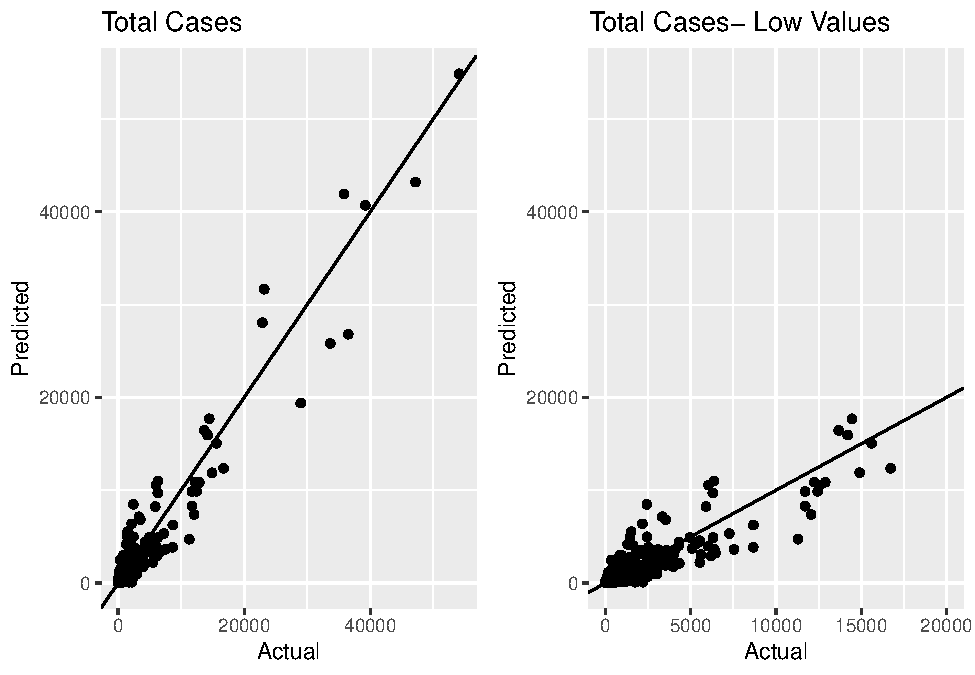
\includegraphics{Final-Project-Covid-19_files/figure-latex/unnamed-chunk-11-1.pdf}
\caption{Fitted vs Actual Total Cases}
\end{figure}

\hypertarget{k-nearest-neighbors}{%
\subsection{K-Nearest Neighbors}\label{k-nearest-neighbors}}

We try k-nearest neighbors technique to predict the number of cases for
counties.We use total number of cases instead of cases per 100K
population. We first use PCA to scale the data and reduce the number of
variables. Using 9 principle components, we select K = 3 from the K-RMSE
plot. The knn model gave us an average out of sample RMSE of 1499. The
RMSE for knn model is around the same level we obtained from negative
binomial model. However, this model does not provide any insight into
the importance of variables in determining the number of cases.

\hypertarget{analysis-using-random-forest-and-boosting-trees}{%
\subsection{Analysis using Random Forest and Boosting
Trees}\label{analysis-using-random-forest-and-boosting-trees}}

We fit random forest and boosting models on cases per 100k population.
By using these models we can also get information about variable
relevance .After a train test split of our sample, we created 1000 trees
by random forest including a minimum of 5 features per bucket.

Table A3 summarizes the variable importance information derived from the
random forest model (RF). We can notice that as expected the population
density per square mile plays an importante role as expected. It
suggests that Counties more dense must expect a higher number of people
infected, as happened in New York state. From the variable importance
table we can also see demograohic and economic covariates of population
that are more likely to be exposed to the virus, such as occupation
type. As mentioned, we fit a Boosting Tree(BT) that allows us to
validate the results of the RF model. The BT model generates a variable
importance output as well, the result in this case are closed with those
released by the RF and are summarized in table A3.

\begin{figure}
\centering
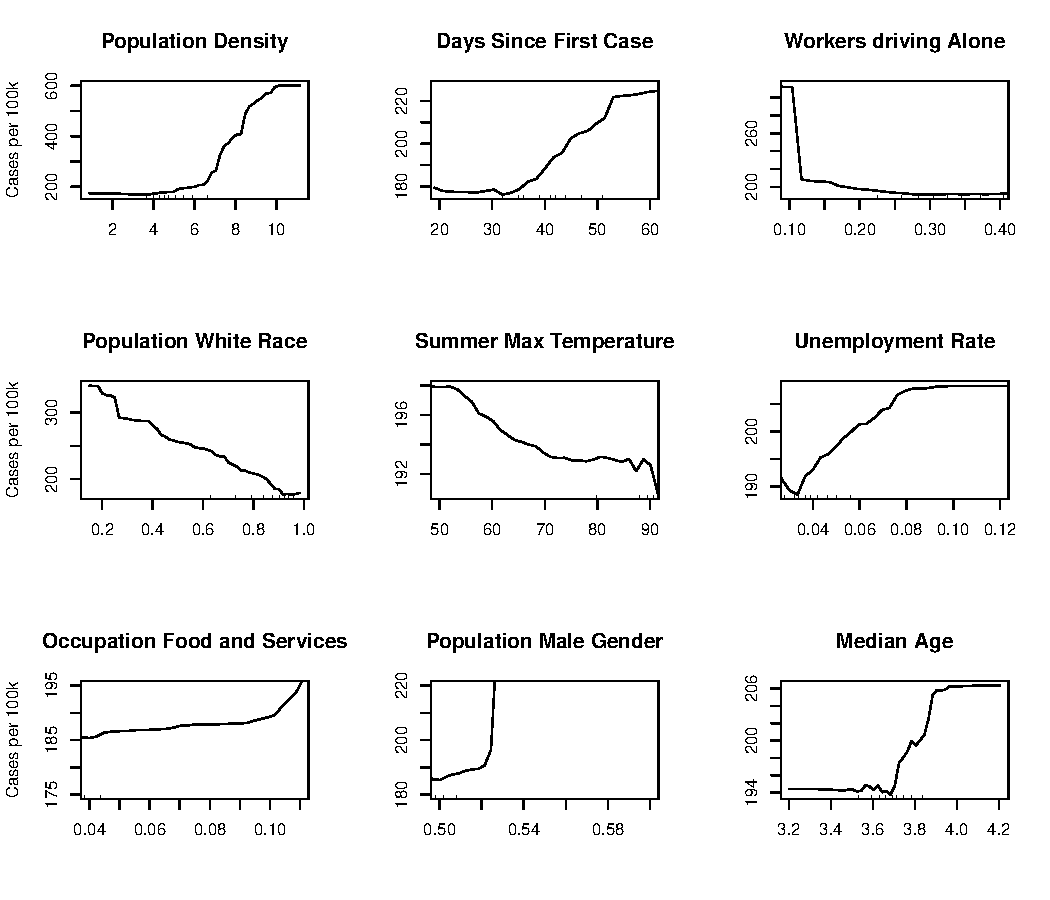
\includegraphics{Final-Project-Covid-19_files/figure-latex/fig1-1.pdf}
\caption{Partial Dependence From Random Forest Model}
\end{figure}

From Random Forest model and Boosting Trees we have the posibility to
generate partial dependence functions. This functions show the marginal
effect of one feature on the predicted outcome of our model. A partial
dependence function can be represented as:

\[\hat{g}_{x_i}(x_i)=E_{X}\left[\hat{g}(x_i,X)\right]=\int\hat{g}(x_i,X)d\mathbb{P}(X)\]

Where \(x_i\) are the variables for which we are computing the function
and matrix X the other variables used in the model \(\hat{g}\). Then,
the partial function tell us for a given value of covariate \(i\) what
the average marginal effect on the prediction is. Then by the
calculation of the partial depence functions we can look for the effect
of the County level features over the number of Covid cases per 100k.
Figure 8 shows the partial depence function derived of the RF for some
features we found intuitive, for example we can observe the can confirm
the positive relation of population density over number of cases. We
also can evaluate the effect of a socioeconomic variable such as poverty
level, specifically we can see that an increase of poverty level has a
positive impact over number of cases. In the case of proportion of
population being white has a negative effect on number of cases. This
finding goes in line with the last reports of New York State that
suggest that the most affected ethnicity or race are Hispanic and Black.
It is also interesting to see how warmer summer temperatures have a
negative effect over Covid cases. Finally, we can see how a higher
median age has a positive effect and more people driving alone to work
has a negative one.

Regarding the predictive performance of tree models, we got an out of
sample RMSE of 247 for the RF model and 301 for the BT. In case of total
cases, we get an out of sample RMSE of around 1400 which is slightly
less than negative binomial and KNN models.

\hypertarget{conclusion}{%
\section{Conclusion}\label{conclusion}}

By running different models on the available data, we were able to
highlight some county level factors that are correlated with the spread
of covid-19 virus. From our analysis, we have gathered that high
population density, lower level of education, higher unemployment,
higher median age, lower proportion of white race and male and more
employment in food, accomodation and health sectors are factors that are
correlated with higher number of cases of covid-19 per 100 thousand
people. All of these models show similar predictive power but we think
it can be further improved by including more counties and including
testing data for county level. With the given data, we conclude that
random forests technique gives us the best predictions.

\newpage

\hypertarget{appendix}{%
\section{Appendix}\label{appendix}}

\hypertarget{a1-list-of-variables}{%
\subsection{A1 List of Variables}\label{a1-list-of-variables}}

\begin{table}[ht]
\resizebox{\textwidth}{!}{%
\centering
\begin{tabular}{rll}
  \hline
 & Name & Description \\ 
  \hline
1 & fips & Unique County Code \\ 
  2 & county & County Name \\ 
  3 & State & State Name \\ 
  4 & cases & Total No of Cases as on April 30, 2020 \\ 
  5 & deaths & Total No of Deaths as on April 30, 2020 \\ 
  6 & days\_first\_case & Total Days since reporting of 1st case \\ 
  7 & Tests\_per\_100K & Total Tests conducted per 100K of Population at State Level \\ 
  8 & Stay\_home\_order & Total Days since issuance of stay at home orders \\ 
  9 & Adults\_Bachelor\_degree\_or\_higher & \% of Adults with bachelors or higher degree \\ 
  10 & Unemployment\_rate\_2018 & Unemployment rate \\ 
  11 & Population\_age\_18to64 & \% of Population between age 18 \& 64 \\ 
  12 & Total\_Pop\_SEX\_Male & \% of Population male \\ 
  13 & Total\_Pop\_RACE\_One\_Race & \% of Population belonging to one race only \\ 
  14 & Total\_Pop\_RACE\_White & \% of Population belonging to white race \\ 
  15 & Total\_Pop\_in\_Households\_Householder\_Spouse & \% of Population living in households with spouse \\ 
  16 & Total\_Pop\_in\_Households\_Householder\_Parent & \% of Population living in households with parents \\ 
  17 & Total\_Pop\_Over\_15\_Divorced & \% of Population over 15 divorced \\ 
  18 & Occ\_Administrative\_Waste\_Management & \% of employment in administrative \& waste management \\ 
  19 & Occ\_Educational & \% of employment in educational services \\ 
  20 & Occ\_Healthcare & \% of employment in heath care sector \\ 
  21 & Occ\_Arts\_Entertainment\_Recreation & \% of employment in arts and recreational sector \\ 
  22 & Occ\_Accommodation\_Food\_Services & \% of employment in accomodation and food services \\ 
  23 & Occ\_Other\_Services & \% of employment in other services \\ 
  24 & Occ\_Public\_Administration & \% of employment in Public administration \\ 
  25 & Total\_Workers\_Over\_16 & \% of Total Population above 16 and working \\ 
  26 & Total\_Workers\_Over\_16\_Drove\_Alone & \% of Total Population above 16 and working \\
& &  that drove alone to work \\ 
  27 & Total\_Households\_TYPE\_Family & \% of total households categorized as Family \\ 
  28 & Households\_with\_incomes & \% of total households with incomes \\ 
  29 & Total\_poverty & \% of Population in Poverty \\ 
  30 & summer\_tmmx & 8 Year average maximum summer humidity \\ 
  31 & summer\_rmax & 8 Year average maximum summer temperature \\ 
  32 & Population\_density\_per\_sqrm & Population density per square mile of area \\ 
  33 & Median\_Age & Median age (log) \\ 
  34 & Median\_Household\_Income & Median household incone (log) \\ 
  35 & Total\_Population & Total Population of County (log) \\ 
  36 & workplaces\_percent\_change\_from\_baseline & Total \% decrease in movement to workplaces from \\
& &  the baseline. Based on daily average of 20-29 April  \\ 
  37 & cases100k & Log count of total Cases \\ 
   \hline
\end{tabular}}
\end{table}

\newpage

\hypertarget{a2-summary-of-negative-binomial-model}{%
\subsection{A2 Summary of Negative Binomial
Model}\label{a2-summary-of-negative-binomial-model}}

\begin{table}[ht]
\centering
\begin{tabular}{rrrrr}
 \hline
\multicolumn{4}{c}{vglm(formula = cases100k ~ ., family = pospoisson(), data = covid3)} \\  
 \hline
 & Estimate & Std. Error & z value & Pr($>$$|$z$|$) \\ 
  \hline
(Intercept) & -34.95 & 0.55 & -64.10 & 0.00 \\ 
  days\_first\_case & 0.01 & 0.00 & 26.92 & 0.00 \\ 
  Tests\_per\_100K & 0.00 & 0.00 & 148.86 & 0.00 \\ 
  Stay\_home\_order & -0.01 & 0.00 & -47.32 & 0.00 \\ 
  Adults\_Bachelor\_degree\_or\_higher & -4.19 & 0.05 & -79.67 & 0.00 \\ 
  Unemployment\_rate\_2018 & -2.80 & 0.25 & -11.00 & 0.00 \\ 
  Population\_age\_18to64 & -4.56 & 0.13 & -35.58 & 0.00 \\ 
  Total\_Pop\_SEX\_Male & 12.08 & 0.21 & 58.44 & 0.00 \\ 
  Total\_Pop\_RACE\_One\_Race & 13.42 & 0.21 & 64.49 & 0.00 \\ 
  Total\_Pop\_RACE\_White & -1.94 & 0.02 & -102.95 & 0.00 \\ 
  Total\_Pop\_in\_Households\_Householder\_Spouse & -1.64 & 0.05 & -30.81 & 0.00 \\ 
  Total\_Pop\_in\_Households\_Householder\_Parent & 9.42 & 0.59 & 16.06 & 0.00 \\ 
  Total\_Pop\_Over\_15\_Divorced & -7.38 & 0.21 & -35.98 & 0.00 \\ 
  Occ\_Administrative\_Waste\_Management & -10.70 & 0.59 & -18.13 & 0.00 \\ 
  Occ\_Educational & 2.21 & 0.22 & 9.87 & 0.00 \\ 
  Occ\_Healthcare & 7.48 & 0.18 & 40.92 & 0.00 \\ 
  Occ\_Arts\_Entertainment\_Recreation & -5.15 & 0.50 & -10.23 & 0.00 \\ 
  Occ\_Accommodation\_Food\_Services & -18.92 & 0.34 & -56.05 & 0.00 \\ 
  Occ\_Other\_Services & -25.74 & 0.68 & -37.89 & 0.00 \\ 
  Occ\_Public\_Administration & -2.61 & 0.20 & -12.86 & 0.00 \\ 
  Total\_Workers\_Over\_16 & -1.23 & 0.06 & -21.31 & 0.00 \\ 
  Total\_Workers\_Over\_16\_Drove\_Alone & 1.97 & 0.06 & 31.39 & 0.00 \\ 
  Total\_Households\_TYPE\_Family & -3.07 & 0.07 & -41.66 & 0.00 \\ 
  Households\_with\_incomes & 7.01 & 0.09 & 79.18 & 0.00 \\ 
  Total\_poverty & 6.39 & 0.10 & 63.86 & 0.00 \\ 
  summer\_tmmx & -0.01 & 0.00 & -11.23 & 0.00 \\ 
  summer\_rmax & -0.00 & 0.00 & -5.59 & 0.00 \\ 
  Population\_density\_per\_sqrm & 0.21 & 0.00 & 76.21 & 0.00 \\ 
  Median\_Age & 2.73 & 0.05 & 55.78 & 0.00 \\ 
  Median\_Household\_Income & 1.35 & 0.03 & 51.87 & 0.00 \\ 
  workplaces\_percent\_change\_from\_baseline & -5.41 & 0.05 & -118.65 & 0.00 \\ 
  \hline
 \multicolumn{1}{r}{Name of linear predictor} & \multicolumn{4}{l}{loglink(lambda)}\\
 \multicolumn{1}{r}{Log-likelihood} & \multicolumn{4}{l}{-96986.51 on 1411 degrees of freedom} \\
 \multicolumn{1}{r}{Number of Fisher scoring iterations} & \multicolumn{4}{l}{10} \\
 \multicolumn{1}{r}{Hauck-Donner effect} & \multicolumn{4}{l}{(Intercept)  Population-age-18to64 summer-tmmx} \\
\hline
   
\end{tabular}
\end{table}

\newpage

\hypertarget{a3-variable-importance-random-forest-and-boosting-tree}{%
\subsection{A3 Variable Importance Random Forest and Boosting
Tree}\label{a3-variable-importance-random-forest-and-boosting-tree}}

\begin{table}[ht]
\centering
\begin{tabular}{lcc}
  \hline
Variable & Boosting Tree (Rel.inf) & Random Forest \\ 
  \hline
Population\_density\_per\_sqrm & 25.10 & 19.15 \\ 
Total\_Pop\_SEX\_Male & 17.21 & 1.69 \\ 
Occ\_Accommodation\_Food\_Services & 10.57 & 10.14 \\ 
Total\_Pop\_Over\_15\_Divorced & 7.59 & 7.44 \\ 
Tests\_per\_100K & 6.02 & 23.43 \\ 
Occ\_Other\_Services & 5.74 & 5.26 \\ 
Total\_Pop\_RACE\_White & 4.00 & 13.27 \\ 
Median\_Household\_Income & 3.21 & 7.63 \\ 
 workplaces\_percent\_change\_from\_baseline & 2.73 & 9.92 \\ 
 Total\_Pop\_in\_Households\_Hh_Spouse & 2.56 & 9.80  \\ 
 Total\_Pop\_in\_Households\_Hh\_Parent & 1.38 &  14.31 \\ 
  Stay\_home\_order & 1.33 & 10.26  \\ 
  Occ\_Educational & 1.27 & 8.26\\ 
  summer\_tmmx & 1.26 & 11.57 \\ 
  Total\_Households\_TYPE\_Family & 1.11 & 6.83\\ 
  Adults\_Bachelor\_degree\_or\_higher & 1.10 & 8.61\\ 
  Days\_first\_case & 0.91 & 9.11 \\ 
  opulation\_age\_18to64 & 0.88 & 9.96 \\ 
  Households\_with\_incomes & 0.80 & 9.42 \\ 
  Occ\_Administrative\_Waste\_Management & 0.73 & 5.30 \\ 
  Median\_Age & 0.60 & 8.20 \\ 
  Total\_poverty & 0.59 & 6.29 \\ 
  Occ\_Healthcare & 0.58 & 8.01 \\ 
  Occ\_Public\_Administration & 0.47 & 1.52 \\ 
  Total\_Workers\_Over\_16 & 0.43 & 8.11 \\ 
  Total\_Pop\_RACE\_One\_Race & 0.42 & 7.37 \\ 
  summer\_rmax & 0.37 & 6.51 \\ 
  Occ\_Arts\_Entertainment\_Recreation & 0.37 & 4.99 \\ 
  Total\_Workers\_Over\_16\_Drove\_Alone & 0.34 & 7.57 \\ 
  Unemployment\_rate\_2018 & 0.34 & 6.80 \\ 
   \hline
\end{tabular}
\end{table}

\newpage

\end{document}
